\usetikzlibrary{calc}
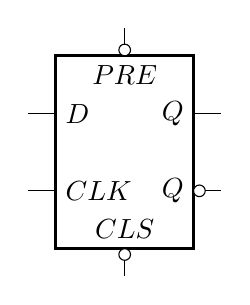
\begin{tikzpicture}[scale=0.7]
  \def\w{2.5}
  \def\h{3.5}
  \draw[line width=1.2] (0, 0) rectangle (\w, \h);

  \draw ($(0, 0)!0.7!(0,\h)$) coordinate (d) -- ++(left:0.5);
  \draw ($(0, 0)!0.3!(0,\h)$) coordinate (clk) -- ++(left:0.5);
  \draw ($(\w, 0)!0.7!(\w,\h)$) coordinate (q) -- ++(right:0.5);
  \draw ($(\w, 0)!0.3!(\w,\h)$) coordinate (nq) -- ++(right:0.5);
  \draw (\w/2, \h) coordinate (pre) -- ++(up:0.5);
  \draw (\w/2, 0) coordinate (cls) -- ++(down:0.5);

  \node[below] at (pre) {$PRE$};
  \node[above] at (cls) {$CLS$};
  \node[right] at (d) {$D$};
  \node[right] at (clk) {$CLK$};
  \node[left] at (q) {$Q$};
  \node[left] at (nq) {$Q$};

  \draw[fill=white,draw=black] ($(nq)+(3pt,0)$) circle (3pt);
  \draw[fill=white,draw=black] ($(pre)+(0,3pt)$) circle (3pt);
  \draw[fill=white,draw=black] ($(cls)-(0,3pt)$) circle (3pt);
\end{tikzpicture}
